%\documentclass[12pt]{article}
\documentclass[12pt]{book} % for chapters
%\usepackage{fullpage}
%\usepackage[top=1in,bottom=1in,left=1in,right=1in]{geometry}
\usepackage[margin=1in, paperwidth=8.5in, paperheight=11in]{geometry}
\usepackage[english]{babel}
\usepackage[utf8x]{inputenc}
\usepackage{amsmath}
\usepackage{graphicx}
\usepackage{caption}
\usepackage[depth=subsection]{bookmark}
\usepackage{multirow}
\usepackage[usestackEOL]{stackengine}
%https://www.sharelatex.com/learn/Code_listing
%For code view in latex

\usepackage{pdflscape}

\usepackage{listings}


%\usepackage[linktocpage=true]{hyperref}
\hypersetup{
    pdfborder = {0 0 0}
}

\usepackage[colorinlistoftodos]{todonotes}
\usepackage{chngcntr}
\usepackage{url}
%header and footer package
\usepackage{fancyhdr}
\usepackage[en-US]{datetime2}

%clearing default page heading and footer
\pagestyle{fancy}



\fancyhf{}
%
\ifx
     E for even page
    O for odd page
    L for left side
    C for centered
    R for right side 
\fi
\lfoot{\fancyfoot[LE,LO]{\leftmark}} 
\rfoot{ PAGE - \thepage} 



\fancyhead{}
\renewcommand{\footrulewidth}{1pt}
\renewcommand{\headrulewidth}{0pt}
\parindent 0ex
\renewcommand{\baselinestretch}{1.5}

% Redefine the plain page style
\fancypagestyle{plain}{%
    \lfoot{\fancyfoot[LE,LO]{\leftmark}} 
    \rfoot{ PAGE - \thepage} 
}




\begin{document}


\begin{titlepage}

\newcommand{\HRule}{\rule{\linewidth}{0.5mm}} % Defines a new command for the horizontal lines, change thickness here
\center % Center everything on the page
 
%----------------------------------------------------------------------------------------
%	HEADING SECTIONS
%----------------------------------------------------------------------------------------

\textsc{\Large Department of Computer Science \& Engineering}\\[0.5cm] % Name of your university/college
\textsc{\Huge United International University}\\[1cm] % Name of your university/college
 %\textsc{\Large Major Heading}\\[0.5cm] % Major heading such as course name
 % \textsc{\large Minor Heading}\\[0.5cm] % Minor heading such as course title

%----------------------------------------------------------------------------------------
%	TITLE SECTION
%----------------------------------------------------------------------------------------

\HRule \\[0.4cm]
{ \huge \LARGE \textbf{CSE6001: Advanced Database Systems}}\\ [0.4cm] % Title of your document
{ {\Large \textbf{Database Privacy and Security: Concepts, Risks and Practices}}}\\
\HRule \\ [1cm]
%  \textit{A dissertation submitted to the United International University in partial fulfillment of the
% requirement for the degree B. Sc. in Computer Science \& Engineering}
%----------------------------------------------------------------------------------------
%	AUTHOR SECTION
%----------------------------------------------------------------------------------------


\begin{minipage}{0.5\textwidth}
\begin{flushleft} \small
\emph{\textbf{\large Author}:}\\

Mohammad Saifur Rahman\\
ID : 0122420002\\
Ekra Hossain\\
ID : 0122420004\\
S.M. Absar Rashid\\
ID : 0122420025\\
SHAMS AREFIN RUBAIYAT\\
ID : 0122420040\\




\end{flushleft}
\end{minipage}
~
\begin{minipage}{0.4\textwidth}
\begin{flushright} \large
\emph{\textbf{Supervisor}:} \\
\small
Dr. Mohammad Rezwanul Huq  \\% Supervisor's Name
Associate Professor \\
Department of CSE, EWU\\

\end{flushright}
\end{minipage}\\[3cm]

% If you don't want a supervisor, uncomment the two lines below and remove the section above
%\Large \emph{Author:}\\
%John \textsc{Smith}\\[3cm] % Your name

%----------------------------------------------------------------------------------------
%	DATE SECTION
%----------------------------------------------------------------------------------------

\ifx
\textregistered\textcopyright
\sffamily\textregistered\textcopyright
\fi

Copyright\textcopyright{Year \the\year}\\
%{\large \today}\\[2cm] % Date, change the \today to a set date if you want to be precise
\DTMlangsetup{showdayofmonth=false}
\today\\[1cm]
%----------------------------------------------------------------------------------------
%	LOGO SECTION
%----------------------------------------------------------------------------------------


\includegraphics[width=100px]{assets/uiu-logo.png}\\[1cm] % Include a department/university logo - this will require the graphicx package
 
%----------------------------------------------------------------------------------------

\vfill % Fill the rest of the page with whitespace

\end{titlepage}


%=========COVER PAGE ENDS HERE==========================
%=========COVER PAGE ENDS HERE==========================



\pagenumbering{roman}




%==================Table of contents PAGE starts HERE=============
%==================Table of contents PAGE starts HERE=============
%\frontmatter
\pagenumbering{arabic}
\counterwithin{equation}{chapter}
% \counterwithin{figure}{chapter}






% \thispagestyle{empty}
%     \addtocontents{toc}{\protect\thispagestyle{empty}}
% \tableofcontents
% \thispagestyle{empty}
% \clearpage

%\addtocontents{toc}{~\vfill}
\addtocontents{toc}{~\hfill{\large \textbf{Chapters}}}
\addtocontents{toc}{~\hfill{\large \textbf{Page}}\par}

%==================Table of contents PAGE ends HERE=============
%==================Table of contents PAGE ends HERE=============




\setcounter{page}{1}


% Points to be focused: Term Paper
% ===============================
% Texonomy
% general classification
% tree
% hiararchy
% comparison
% related work comparison
% workflow
% more figure

%=================Introduction PAGE Starts HERE=================
%=================Introduction PAGE Starts HERE=================

\section*{Abstract}

This paper represents a extensive review of security measures in database systems, focusing on authentication, access control, encryption, auditing, intrusion detection, and privacy-enhancing techniques. It's focus to provide fresh perspective into the recent developments and recommended guidelines in securing databases. The review  explores the obstacles, vulnerabilities, and risk reduction plans associated with 
database security. It examines a range of authentication approaches, access control models, encryption techniques, auditing and monitoring approaches, threat detection systems, and data breach prevention strategies. The paper additionally analyzes the implications of emerging trends such as cloud computing, big data database security. By surveying previous studies, this review seeks to further the development of database security and support organizations in protecting their valuable data.\cite{a_comprve_rev_of_sec_measr_in_db_sys_assess_auth_accss_ctrl_bynd} \label{sec:a_comprve_rev_of_sec_measr_in_db_sys_assess_auth_accss_ctrl_bynd_1}\\

\section*{Introduction}

%Introduction PAGE ends HERE----------
%Introduction PAGE ends HERE----------

\subsection*{Common Database Security Issues}


Data corruption due to the entering invalid data and or commands, also mistake in the database can result weakness in database or repository systems. According to the NCC Group Study, UK following are the common
database security issues.\cite{db_security_an_overview_and_analysis_of_current_trend} \label{sec:db_security_an_overview_and_analysis_of_current_trend_1}\\

\begin{figure}[h]
	\begin{center}
	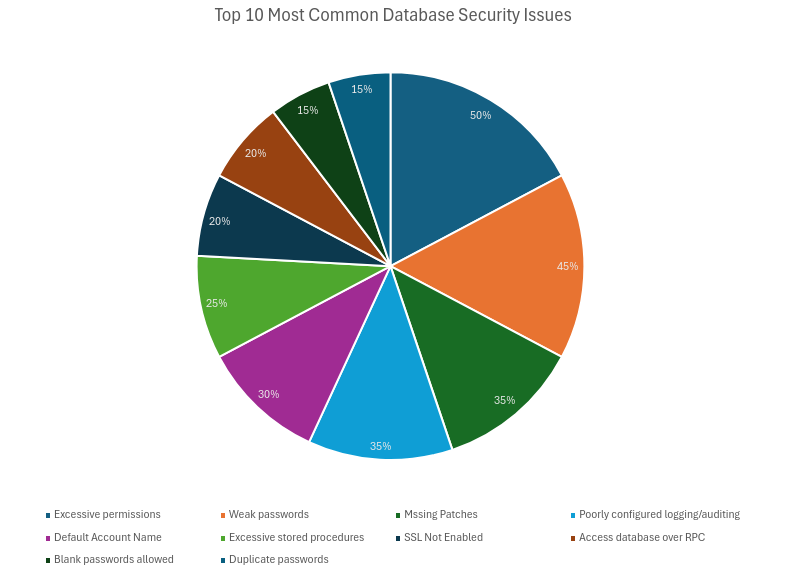
\includegraphics[width=0.8\textwidth]{assets/top_10_most_common_db_security_issues.png}
	\end{center}
	%latex how to skip a figure in list of figure
	\caption[]{Some of the common Database Security
    Survey (NCC Group Survey, UK)}
	\label{fig:top_10_most_common_db_security_issues}
\end{figure}


\subsection*{Types of Database Security}

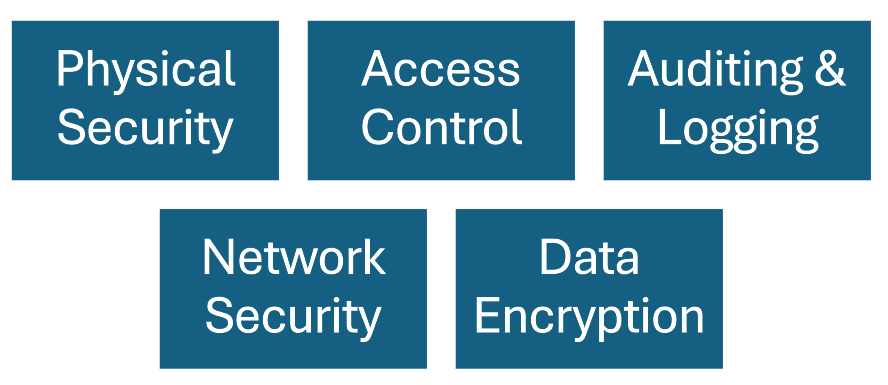
\includegraphics[width=450px]{assets/types_of_db_security.png}\\[1cm] % Include a department/university logo - this will require the graphicx package





\begin{itemize}
		\item \textbf{Physical Security:} Physical Security means protecting database from unauthorized access physical level. This means applying security in server rooms, monitoring who has previleges and enter the data center, and also using enough security cameras and alarming systems.
		
		
		\item \textbf{Access control:} Access control states that Implementing restrictions database access to authorized users only. It includes several key components, authentication, authorization.

        \item \textbf{Network Security:} Network Security implies preventing harm to the database from unauthorized access and keeping the database safe from network-based threats. 
        
        There are several Key measures we can take like firewalls, intrusion detection systems, encryption, Virtual Private Networks, Access Control, Network Segmentation, Patch Management, Secure Network Protocols, DDoS Protection, Network Monitoring, User Education and Awareness, Zero Trust Security and so on.
\end{itemize}





\renewcommand\bibname{References} % Removing thebibliography title
\begin{thebibliography}{1}
\addcontentsline{toc}{chapter}{\refname} %make bibliography as reference chapter 

    \bibitem{db_security_an_overview_and_analysis_of_current_trend}  \hyperref[sec:db_security_an_overview_and_analysis_of_current_trend_1]{P. K. Paul, and P. S. Aithal, ``Database Security: An Overview and Analysis of Current Trend"} 

    \bibitem{a_comprve_rev_of_sec_measr_in_db_sys_assess_auth_accss_ctrl_bynd}  \hyperref[sec:a_comprve_rev_of_sec_measr_in_db_sys_assess_auth_accss_ctrl_bynd_1]{Habeeb O., and Maryam
A., ``A Comprehensive Review of Security Measures in Database Systems: Assessing Authentication, Access Control, and Beyond"} 

   

% A. Hamza, and B. Kumar, "A review paper on DES, AES, RSA encryption standards." pp. 333-338.
    % \bibitem{purchase_module_book}  \hyperref[sec:purchase_module_book_1]{Mitchell, V. \& Simpson, D.F. (2007). R12 Oracle purchasing fundamentals.} 
    % \bibitem{sql_book} \hyperref[sec:sql_book_1]{Clement, S. \& Pottle, B. \& Singh, P. (2010). Oracle Database: SQL Fundamentals I.}
    % \bibitem{sql_book2} \hyperref[sec:sql_book_1]{Koratamaddi, C. \& Pottle, B. \& Srivastava, T. (2010). Oracle Database: SQL Fundamentals II.}
    
    % \bibitem{plsql_book} \hyperref[sec:plsql_book_1]{Pottle, B. (2009). Oracle Database 11g: PL/SQL Fundamentals.}
    % \bibitem{plsql_book2} \hyperref[sec:plsql_book_1]{Serhal, L.K. (2009). Oracle Database 11g: Develop PL/SQL Program Units.}
    
    % \bibitem{form_builder_book}  \hyperref[sec:form_builder_book_1]{Gamer, P. (2006). Oracle Forms Developer 10g: Build Internet Applications.}
    
    % \bibitem{norman} \textit{Oracle Purchasing User's Guide}. (2018, January 10). Retrieved  from  {\url{https://docs.oracle.com/cd/E18727_01/doc.121/e13410/toc.htm}}
    
    % \bibitem{norman} Greenwood, S. (August 3, 2015). The future of Oracle Forms. Retrieved  from  {\url{http://www.explorer.uk.com/the-future-of-oracle-forms/}}
    
    % \bibitem{feature_forms} \hyperref[sec:feature_forms_1]{ \textit{The future of Oracle Forms}. (2018, February 10). Retrieved  from  {\url{https://www.toadworld.com/platforms/oracle/w/wiki/11125.the-future-of-oracle-forms}} }
  
\end{thebibliography}
  


\end{document}
